\chapter{Design \& Model}
\label{chap:model}

We now present our design and model for mixed-criticality scheduling support in a high-assurance
system such as \selfour. 

Our goal is to provide support in the kernel for mixed-criticality workloads.  This involves
supporting tasks of different time sensitivity, (\gls{HRT}, \gls{SRT}, best-effort), different
criticalities, and different levels of trust.  Such tasks should not be forced into total
isolation, but be permitted to share resources without violating their temporal correctness
properties through mechanisms provided by the kernel.

To achieve this we require temporal isolation: a feature of resource kernels, whose mechanisms we
apply to our research platform, \selfour.  However temporal isolation is not enough: mixed-criticality
systems require asymmetric protection rather than temporal isolation, as a result we leverage
traditional resource kernel reservations but decouple them from priority, allowing the processor to
be overcommitted while providing guarantees for the highest priority tasks.

In this section we first address how we integrate resource kernel mechanisms with \selfour with
mechanisms for temporal isolation. We then describe our mechanisms for temporal isolation of
resources shared between clients of different levels of criticality, time sensitivity, and trust.
Finally, we show how our mechanisms can be used to build several existing user-level policies. 

Our design goals are as follows:
\begin{description}\sloppy
    \item[Capability-controlled enforcement of time limits:] In general, capabilities
      help to reason about access rights. Furthermore, they allow a
        seamless integration with the existing capability-based spatial
          access control of security-oriented systems such as \selfour.
    \item[Policy freedom:] In line with microkernel philosophy
        \citep{Heiser_Elphinstone_16}, the model should not force systems
        into a particular resource-management policy. In particular, it
        should support a wide range of scheduling policies and
        resource-sharing models, such as locking protocols.
    \item[Efficient:] The model should add minimal overhead over the best
                      existing implementations. In particular, it should be compatible
                        with fast IPC implementations in high-performance microkernels.

    \item[Temporal isolation:] The model must allow system designers to create systems where a
        temporal failure in one component cannot cause a temporal failure in another part of the
        system.

    \item[Overcommitment:] The model must allow systems to be specified that are not necessarily
        schedulable: as the degree and nature of overcommitment is a core policy of a particular
        system. Overcommitment is also key to providing  asymmetric protection, where high
        criticality tasks can disrupt low criticality tasks.

    \item[Safe resource sharing:] Temporal isolation should persist even in the case of
        shared-resources, to provide mechanisms for sharing between applications with different
        levels of time-sensitivity, criticality and trust.
\end{description}

The model  provides temporal isolation mechanisms from the kernel, while allowing for more complex
scheduling policies to be implemented at user level.

\section{Scheduling}

We outlined four core resource kernel mechanisms---admission, scheduling, enforcement and
accounting---that are essential to resource kernels for implementing temporal isolation.  However,
as noted in \Cref{sec:resource-kernels}, such kernels are monolithic, where all policy, drivers and
mechanisms are provided by the kernel.

Microkernels like \selfour offer a different design philosophy, based on the principle of
minimality~\citep{Liedtke_95}, where mechanisms are only included in the kernel if they would
otherwise prevent the implementation of required functionality. Previous resource kernels
are all monolithic, where all resource policies are implemented in the kernel itself.

The goals of resource kernels do not directly align with that of microkernels in general.  This is
because microkernels do not directly manage all resources in the system, but provide mechanisms for
the system designer to implement custom resource management policies.  

In \selfour, mechanisms for physical memory, device memory, interrupt and \IO port management are
exposed to the user via the capability system, as outlined in \cref{chap:sel4}. As a result, the
only resource that the kernel needs to provide reservations for is processing time.  We now present
our mechanisms, and discuss how each of the four resource kernel policies can be implemented within our model.

\subsection{Scheduling}
\label{sec:model-scheduling}

There are two design choices relevant to scheduling:

\begin{itemize} 
    \item Should a scheduler be provided in the kernel at all? 
    \item Should the scheduling algorithm be fixed (\gls{FP}) or dynamic (\gls{EDF}) priority?
\end{itemize}

\subsubsection{Kernel scheduling}

We retain the scheduler in the kernel, unlike \composite, for two reasons: to
maintain a small trusted computing base, and for performance. Any system with
multiple threads of execution, which is required in a mixed-criticality system,
must have a scheduler, which for the purposes of temporal isolation is part of
the trusted computing base. If a system must have a scheduler, and in a
mixed-criticality system, with untrusted components, that scheduler must be in
a separate protection domain to those untrusted components, then a scheduling
decision will require at least two context switches: from the preempted thread
to the scheduler, and from the scheduler to the chosen thread. Placing a basic
scheduler in the kernel reduces this overhead. 

Additionally, as the scheduler is a core component of the system it must be
verified: by keeping the
scheduler in the kernel we maintain the current verification. Verification of a user-level scheduler
and its interaction with the kernel is a far more complex task, especially as verification of
concurrent systems is very much an open research challenge. 

One might claim maintaining a scheduler in the kernel is a violation of our goal of policy freedom.
However, we maintain this is not the case, which comes down to our choice of fixed priorities over
\gls{EDF}.

\subsubsection{Fixed priorities}

Our model uses \gls{FP} scheduling as a core part of the kernel, with the addition of mechanisms
that allow for the efficient implementation of user-level schedulers.
We choose \gls{FP} over \gls{EDF} for three reasons; 
fixed-priority is dominant in industry
as shown in \cref{chap:operating-systems} and maps well to \gls{FP} with \gls{RM} priority assignment; and dynamic scheduling policies like
\gls{EDF} can be implemented at user level; and \gls{FP} has defined behaviour on overcommitted
systems.

\gls{EDF} scheduling can be implemented by using a single priority for the dynamic
priorities of \gls{EDF}, as we will demonstrate in \cref{s:edf-impl}.
However, the opposite is not true: mapping the dynamic priorities of EDF to a fixed-priority
is non-trivial and would come with high overheads. 
Our approach is consistent with existing designs in Linux  and ADA~\citep{Burns_Wellings:crtpa}, which
support both scheduling algorithms, usually with \gls{EDF} at a specific priority. Additionally,
schedulability analysis of \gls{EDF}-within-priorities is well
understood~\citep{Harbour_Palencia_03}.

We do not consider Pfair scheduling (recall \cref{s:pfair}) an option, as its high interrupt
overheads and fairness properties are not suitable for hard real-time systems.  Again however, it is
possible to implement a Pfair scheduler at user level.

The final reason to base the approach on fixed priorities is the ability
to reason about the behaviour of an
overcommitted system. Overcommitting, is important for achieving high
actual system utilisation, given the large time buffers required by
critical hard real-time threads. It is also essential to keeping the kernel
policy-free: The degree and nature of overcommitment is a core policy
of a particular system. For example, the policy might require that the
total utilisation of all \crit{high} threads is below the \gls{FPRM}
schedulability limit of 69\%, while \crit{low} threads can overcommit,
and the degree of overcommitment may depend on the mix of hard RT,
soft RT and best-effort threads. Such policy should be defined and
implemented at user level rather than in the kernel.

As discussed in \autoref{s:overload}, the result of overload in an
EDF-based system is hard to predict, and such a system is hard to
analyse. In contrast, with fixed priority the result is easy to
understand: If the sum of utilisations of threads at priority \(\geq
P\) is below the utilisation bound, then all those threads will meet
their deadlines, while any thread with priority \(<P\) may miss. This
allows easy analysis of schedulability, including when the system
criticality changes.

\subsection{Scheduling contexts}
\label{sec:model-scheduling-contexts}

At the core of the model is the \emph{\gls{SC}} as the
fundamental abstraction for time allocation, and the basis of 
the enforcement and accounting mechanisms in our model.
A \gls{SC} is a representation
of a reservation in the object-capability system, which means that 
they are first-class objects, like threads, address spaces, or
\gls{IPC} endpoints. An SC is represented by a capability to a
scheduling context object.

In order to run, a thread needs an \gls{SC}, which represents the
maximum CPU bandwidth the thread can consume. Threads obtain \glspl{SC} through \emph{binding}, and
only one thread can be bound to an \gls{SC} at a time, to avoid hierarchical scheduling.
In a multicore system, an SC represents the right to access a
particular core. Core migration, e.g.\ for load balancing, is policy
that should not be imposed by the kernel but implemented at user
level. A thread is migrated by replacing its SC with one tied to a
different core. This renders the kernel scheduler a partitioned scheduler, 
which aligns with our efficiency goal; partitioned schedulers outperform global
schedulers~\citep{Brandenburg:phd}.

The unfungible nature of time in real-time systems requires that the
bandwidth limit must be enforced within a certain time window. We
achieve this by representing an SC by sporadic task parameters, \emph{period}, \(T\), and a
\emph{budget}, \(C\), where \(C\leq T\) is the maximum amount of time
the SC allows to be consumed in the period. \(U=\frac{C}{T}\) represents the
maximum \emph{CPU utilisation} the SC allows. The SC can be viewed as
a generalisation of the concept of a time slice, discussed in \cref{s:timeslices-and-meters}.

In order to support MCS, we do not
change the meaning of priority, but what it means for a thread to be
\emph{runnable}: We associate each thread with an SC, and
make it non-runnable if it has exhausted its budget. 


\glspl{SC} can be gracefully integrated into the 
existing model used in \selfour,
logically replacing the time slice attribute with the scheduling context object.

Unlike \fiascooc's scheduling contexts~\citep{Lackorzynski_WVH_12}, which
are superficially similar to ours, we retain priorities as a thread
attribute rather than making them part of \glspl{SC}\footnote{\fiascooc's scheduling
contexts are not integrated in to the capability system.}. The advantage of keeping the two
orthogonal will become evident in \cref{s:locking}.

\subsection{Accounting}
\label{sec:model-accounting}

Accounting must be a mechanism implemented by the kernel, as the kernel is the only entity in the system
that can monitor all threads, regardless of preemption in the system, since the kernel facilitates all
preemption.
The accounting mechanism is provided by new system invariant that the currently running thread 
must have a scheduling context with available budget, as all time consumed is billed to the
current scheduling context.
This includes time spent executing in the kernel, including preemptions.
The rule for accounting kernel time is all time, from kernel entry, is billed to the scheduling
context active on kernel exit. This means that if a thread is preempted and 
that preemption does not trigger a switch to a 
different scheduling context, all time is accounted to the current scheduling context. Otherwise, 
time from kernel entry is accounted to the next scheduling context.

In order to facilitate user-level schedulers, the kernel tracks the amount of time consumed by a
scheduling context, which can be retrieved by an invocation on that specific scheduling context
object.
We specifically do not cater for dynamic frequency scaling and ensure that it is turned off
during testing---this is out of scope and a topic for future work. 

\subsection{Admission control}
\label{sec:model-admission}

Unlike any previous kernel that supports reservations, our model delegates admission control to user
level, as it is deeply tied to policy, which a microkernel should not limit. A consequence of this
choice is the design naturally supports over-commitment, as this is part of the admission test.

The mechanisms for admission control consist of two parts: scheduling contexts are created without
any budget at all, and a new control capability must be invoked to populate scheduling context
parameters.
\schedcontrol is the new control capability, one of which is provided per processing core,
and grants authority to 100\% of time on that core, thus providing the admission-control privilege.
This is analogous to how \selfour controls the right
to receive interrupts, which is controlled by the IRQ\_control
capability as introduced in \cref{s:control-capabilities}. Like time, IRQ sources are non-fungible.

Unlike the reservations in resource kernels, the scheduling context does not 
act as a lower-bound on CPU bandwidth that a thread can consume. This, combined with
user-level admission control, is also key to allowing system designers to over-commit the system. 

By designating admission tests as user-level policy, we allow system designers complete freedom
in determining which admission test to use, if at all, and when that test should be done.
Consequently, they can be run dynamically at run-time, or offline, as per user-level policy.

Thus, the kernel places no restriction on the creation of reservations apart from minor integrity
checks (\ie $C \leq T$).
For example, some high-assurance systems may sacrifice utilisation for safety with a very basic but easily verifiable, online, admission test.
Other implementations may conduct complex admission tests offline in order to obtain the highest possible utilisation, using algorithms that are not feasible at run time.
Some systems may require dynamic admission tests that sacrifice utilisation or have increased risk.
Basic systems may require a simple break up of the processing time into rate-limited reservations.
By taking the admission test out of the kernel, all of these extremes (and hybrids of) are optional policy for the user.

A consequence of this design is that more reservations can be made than processing time available.
This is a desirable feature: it allows system designers to overcommit the system, while features of the scheduling mechanisms provided by the kernel guarantee that the most important tasks get their allocations, if the priorities of the system are set correctly.

However, allowing any thread in the system to create reservations could result in overload behaviour and violation of temporal isolation.
To prevent this, admission control is currently restricted to the task that holds the scheduling
control capability for each processing core.

\subsection{Replenishment}

Scheduling contexts can be \emph{full} or \emph{partial}. A thread with a \emph{full} SC, where
\(C=T\), may monopolise whatever
CPU bandwidth is left over from higher-priority threads, while high-priority threads with full
\glspl{SC} may monopolise the entire system. 
Partial \glspl{SC}, where \(C<T\), are not runnable once
they have used up their budget, until it is replenished, and form our mechanism for temporal
isolation.  

Full \glspl{SC} are key to maintaining policy freedom and performance; while systems
must be able to use our mechanisms to enforce upper bounds on execution, the usage of 
those mechanisms is policy. If a task is truly trusted, no enforcement is required,
as in standard \gls{HRT} systems. They can also be used for best-effort threads which run in slack time.
The \(C\) of a full \gls{SC} represents the timeslice, which once expired results in round robin
scheduling at that priority. Additionally, full \glspl{SC} provide legacy compatibility: setting \(C\ = T =\)
the previous timeslice value results in the same behaviour as the master kernel. 

From a performance perspective full \glspl{SC} prevent mandatory preemption overheads 
that derive from forcing all threads in a system to have a reservation. Threads with a full
budget incur no inherent overhead other than the preemption rate $1/T$.

Threads with \emph{partial} \glspl{SC} have a limited budget, which forms an upper
bound on their execution. For replenishment, we
use the sporadic servers model as described in \cref{p:sporadic} with an
implementation based on the algorithms presented
by~\citet{Stanovic_BWH_10}. 

The combination of full and partial \glspl{SC}  and the ability to overcommit distinguishes our
model from that of resource kernels.

\subsubsection{Sporadic servers}
\label{sec:model-sporadic}

We use sporadic servers as they provide a mechanism for isolation without requiring the kernel
to have access to all threads in the system, unlike other approaches discussed in
\cref{background:fp-isolation}, \eg  priority exchange servers and slack stealing.
Deferrable servers do not require global state but are avoided due to the back-to-back
problem.
Avoiding global, shared-state is required for confidentiality, because access to shared state
has cache effects, which leak information via cache-based timing-channels. In order to maintain these properties,
timing channels must be mitigated through partitions. 
It must be possible to partition a system completely, such that operations in one partition do not
alter the cache state in the other partitions.

Recall that sporadic servers work by preserving the
\emph{sliding window} constraint, meaning that during any time
interval not exceeding the period, no more than $C$ can be consumed.
This stops a thread from saving budget until near the end of its
period, and then running uninterrupted for more than $C$. It is achieved by tracking any leftover
budget when
a thread is preempted at time \(t\), and scheduling a replenishment for time  $t+T$.

In practice, we cannot track an infinite number of
replenishments, so in a real implementation, once the number of
queued replenishments exceeds a threshold, any excess budget is
discarded. If the threshold is one, the behaviour degrades to polling
servers~\citep{Sprunt_SL_89a} where any unused budget is lost and the
thread cannot run until the start of the next period. 

There is an obvious cost to replenishment fragmentation that will
arise from preemptions, and polling servers are more efficient in the
case of frequent preemption \citep{Li_WCM_14}; an arbitrarily high
threshold makes little sense. The optimal value depends on
implementation details of the system, as well as the characteristics
of the underlying hardware.
We therefore make the threshold an attribute of the SC. \glspl{SC} are variably sized,
such that system designers can set this bound per SC. This is a generalisation of the approach used
in Quest-V~\citep{Danish_LW_11}, where \IO reservations are polling servers and other reservations 
are sporadic servers, as policy which can easily be implemented at user-level with variably sized
\glspl{SC}.

\subsection{Enforcement}
\label{sec:model-enforcement}

Threads may exhaust their budgets for different reasons. A budget may
be used to rate-limit a best-effort thread, in which case budget
overrun is not different to normal time-slice preemption of
best-effort systems. A budget can be used to force an untrusted thread
to adhere to its declared WCET. Such an overrun is a contract violation, which may be reason
to suspend the thread or restart its subsystem. Finally, an overrun by
a critical thread can indicate an emergency situation; for example,
critical threads may be scheduled with an optimistic budget to provide
better service to less critical threads, and overrun may require
provision of an emergency budget or a system-criticality change.

Clearly, the handling of overrun is a system-specific policy, and the
kernel should only provide appropriate
mechanisms for implementing the desired policy. Our core mechanism is
the \emph{timeout exception}, which is raised when a thread is
preempted due to budget expiry. To allow the system to handle the exceptions, each thread
is optionally associated with a timeout exception handler, which is
the temporal equivalent to a (spatial) protection exception. When a
thread is preempted, the kernel notifies its handler via an IPC message. The
exception is ignored when the thread has no timeout exception handler, and the thread
can continue to run once its budget is replenished.

The timeout fault
endpoint is separate from the existing thread fault endpoint, as the semantics are different,
because non-timeout faults are not recoverable without the action of another thread. 
While threads are not required to have a fault endpoint, when a fault occurs a thread is always
blocked, as it is no longer in a runnable state. Timeout faults on the other hand are recoverable:
the thread must simply wait until budget replenishment. 

Timeout fault handling threads should have their own \gls{SC} to run on, with enough budget to handle
the fault, otherwise they will not be eligible for selection by the kernel scheduler.

Similar to a page fault handler, timeout fault handlers can be used to adjust thread parameters dynamically as may be required for a \gls{SRT} system, or raise an error.
The handler has a choice of a range of overrun policies, including:
\begin{itemize}
      \item providing a one-off (emergency) budget to the thread and letting it continue,
       \item permanently increasing the budget in the thread's SC,
       \item killing/suspending the thread, and
       \item changing the system criticality level.
       \end{itemize}
Obviously, these are all subject to the handler having sufficient
authority (\eg \schedcontrol).

If a replenishment is ready at the time the budget expires, the thread
is immediately runnable. It is inserted at the end of the ready queue
for its priority, meaning that within a priority, scheduling of
runnable threads is round-robin.

The timeout fault handler is similar to the original KeyKOS~\citep{Bomberger_FFHLS_92} concept of
meters, which was carried through to earlier version of L4 as a \emph{preempter}. The preempter was
invoked every time the timeslice/meter expired to make a scheduling decision. This was abandoned due
to performance reasons. Our approach differs in that timeout fault handlers are optional, so that
they can be used in exceptional scenarios only. However, timeout fault handlers can also be used to
facilitate user-level scheduling, which is now feasible as modern hardware has much faster context
switch times. 

\subsection{Priority assignment}

Assignment of priorities to threads is user-level policy. One approach is to simply use
rate-monotonic scheduling: where priorities are assigned to threads based on their period, and
threads use scheduling contexts that match their sporadic task parameters.  Each thread in the
system will be temporally isolated as the kernel will not permit it to exceed the processing time
reservation that the scheduling context represents.

However, the system we have designed offers far more options than simple rate-monotonic fixed-priority
scheduling.  Policy freedom is retained as reservations simply grant a potential right to processing
time, at a particular priority.  What reservations actually represent is an upper bound on
processing time for a particular thread.  Low priority threads are \emph{not} guaranteed to run if
reservations at higher priorities use all available CPU.  However, threads with reservations at low
priorities will run in the system slack time, which occurs when threads do not use their entire
reservation.

The implication is that a system could use a high range of priorities for rate-monotonic threads,
while best-effort and rate-limited threads run at lower priorities.  Another alternative is to map
user-lever schedulers to specific  priorities, for instance an EDF scheduler. 

\subsection{Asymmetric Protection}

Recall that in a mixed-criticality system, asymmetric protection means that tasks with higher
criticality can cause deadline misses in lower criticality tasks.  Two approaches to mixed
criticality scheduling that provide asymmetric are slack scheduling and
\gls{RTA}~\citep{Burns_Davis_17}.

Under slack scheduling, low-criticality tasks run in slack time of high-criticality tasks.  Our
model supports this easily: high-criticality tasks are given reservations to all processing time at
high priorities, and low-criticality tasks given reservations at a lower priority band.

\gls{RTA} relies on suspending or de-prioritising low-criticality tasks if a high-criticality
task runs for longer than expected.  Simple \gls{RTA} schemes involve two system modes:
a \crit{HI} mode and a \crit{LO} mode, although they have been generalised to
more~\citep{Fleming_Burns_13}.  In \crit{LO} mode, high-criticality tasks run with smaller 
reservations, and the remaining
CPU time is used for low-criticality tasks.  If a high-criticality task does not complete before its
\crit{LO}-mode reservation is exhausted, the system switches to \crit{HI} mode: all low criticality
tasks are suspended.  This is also supported by our model: a high-priority scheduling thread can be
set up to receive temporal faults when a task does not complete before its budget expires.  On a
temporal fault, the scheduling thread can extend the reservation of the high-priority task and
suspend all low priority tasks.

\subsection{Summary}

The scheduling, accounting and enforcement mechanisms presented are sufficient to support temporally
isolated, fixed-priority or \gls{EDF} scheduled real-time threads. By keeping admission control
out of the kernel we preserve policy freedom, while the mechanisms provided allow for a full
resource kernel to be built, or other types of system which require the ability to over-commit.
Additionally, we have maintained
support for best-effort threads, and have added the ability to provide asymmetric protection for
mixed-criticality workloads. 
In the next section, we show how our model provides mechanisms for resource sharing. 

\section{Resource sharing}\label{s:locking}

Reservations through the mechanism of scheduling contexts are not sufficient alone to provide
resource sharing between tasks of different time-sensitivity, criticality, and trust. We now
present how the scheduling context mechanism facilitates resource sharing policies 
in terms of the three core mechanisms ---prioritisation, charging and enforcement---presented 
in \cref{sec:resource-kernels}.

In this section we consider only resources shared by resource servers in an \gls{RPC} style where
servers are scheduled directly as a result of the \gls{RPC}. Other forms of resource sharing, such
as the asynchronous multicast provided by ARINC 653 (\cref{s:arinc}), are possible, but not
relevant, as time is not directly exchanged, and we have already shown how temporal partitioning is possible with
reservations. 

RPC-style shared servers are fundamentally a trusted entity: the client does not resume until the
server replies to a request, and the server may not ever reply. Additionally, the client requires the
server to carry out the operation requested. Consequently, the server takes on the ceiling of the
requirements of all the clients. If a server is shared between trusted and untrusted clients, the
server must be trusted as much as the most trusted client. If a server is shared between \gls{HRT}
and best-effort clients, the server must have the same time sensitivity as the HRT clients: a defined 
\gls{WCET} and bounded blocking behaviour. Finally, the server must be at the highest criticality
level of all clients, however the opposite is not true. If a server has sufficient isolation
properties, then all the clients of that server are not also promoted to the
highest criticality level, which as we know greatly increases the certification burden. 

This asymmetry also holds for trust: a trusted server need not trust its clients,
and the clients need not trust each other. 
Trusted scenarios do not require this level of encapsulation: user-level threads packages can implement
locking protocols with libraries such as \texttt{pthreads}. Therefore, our focus is on temporal
isolation in shared servers beyond strict partitioning, where clients do not trust each other, and
the server does not trust the client.

The proposed model supports shared servers, including scheduler
bypass, through \emph{scheduling context
donation}: a client invoking a server can pass its SC along, so the
server executes on the client's SC, until it replies to the
request. This ensures that the time consumed by the server is billed
to the client on whose behalf the server's work is done. If the scheduling context 
expires, the enforcement mechanism of timeout exceptions can be used to recover the server according 
to server specific policy.

\subsection{Prioritisation}

We indicated in \Cref{sec:model-scheduling-contexts} that scheduling contexts are separate from thread control blocks in
order to support resource sharing. Additionally, unlike previous microkernel designs for \glspl{SC}, priority
remains an attribute of the execution context. Decoupling priority and scheduling context avoids
prior patterns where priority-inheritance is enforced by the kernel. 

The \Gls{IPCP} maps neatly to this model: if server threads are assigned the ceiling protocol of all of
their clients, then when the \gls{IPC} rendezvous occurs and we switch from client to server, the
server's priority is used, a consequence of decoupling priority from the scheduling context.
\gls{IPCP} is also practical: it is mandated by the AUTOSAR standard
(recall \cref{sec:os-autosar}) and is therefore understood well by parts of the industry.

The main drawback of the \gls{IPCP}, namely the requirement that all
lockers' priorities are known \emph{a priori}, is easy to enforce in a
capability-based system: The server can only be accessed through an
appropriate invocation capability, and it is up to the system designer
to ensure that such a capability can only go to a thread whose
priority is known or appropriately controlled.

The choice of the \gls{IPCP} over other fixed-priority protocols, the \gls{PIP} and the \gls{OPCP},
is intentional, and we now present the case against both protocols.

In order to properly support real-time systems, our model orders endpoint queues by priority, rather
than the traditional \gls{FIFO} of L4 kernels. Threads of the same priority remain FIFO. 

\subsubsection{\gls{PIP}}

The major factor in ruling the \gls{PIP} out as a mechanism provided by the microkernel is
performance. Introducing \gls{PIP} would drastically increase scheduler operations on the critical
\gls{IPC} fastpath, as priorities would need to be returned on the reply path. One could take after
Real-time Mach, and provide \gls{PIP} as an optional flag on a message port, thereby retaining
policy freedom, but at a performance cost. Mandating the \gls{PIP}, which incurs a high-preemption
overhead compared to other protocols, would violate both our performance and policy freedom
requirements. 

There is an additional, practical concern, in that the \gls{PIP} does not map well to the existing
capability system. Recall from \cref{p:sel4_ipc} that endpoints have very minimal state\footnote{Which
again contributes to high performance.}, and once an IPC rendezvous has occurred, the caller is
blocked on the resume capability. Consequently, there is \emph{no way to reach the caller} after an 
\gls{IPC} message has been sent. 
Significant changes would be required to the \gls{IPC} model to ensure threads
blocked on resume capabilities could be tracked from the endpoint that the message was sent over.



\subsection{\gls{OPCP}}

Although the \gls{OPCP} offers greater processor utilisation than the \gls{IPCP}, it would require the
kernel to track a system ceiling and also implement priority inheritance, in a form where unrelated
threads may inherit priorities due to a resource access pattern. Both of these mechanisms are
required to implement the \gls{OPCP}, and both would violate confidentiality by altering state 
across partitioned resources.  This is the same reason we exclude
priority-exchange and slack-stealing servers, as discussed in \cref{sec:model-sporadic}.

Although not provided by the kernel, \gls{PIP} and \gls{OPCP} can be implemented a user-level if
required, by proxying requests to shared resources via an endpoint and thread which manipulates the priorities
appropriately, before forwarding on the request. For \gls{PIP}, only one extra thread per resource would 
be required and could exist in the same address space as the resource.
Since \gls{OPCP} requires global state, an implementation would require a shared service for all threads 
sharing a set of resources. We describe such an implementation in \cref{sec:model-mechanisms} after introducing further mechanisms
in \cref{sec:model-policies}.

\subsection{Charging}

\begin{figure}
    \centering
    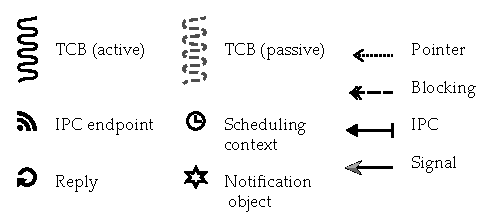
\includegraphics[width=0.7\textwidth]{legend-full}
    \caption[Legend for diagrams in this chapter.]{Legend for diagrams in this chapter, an expanded version of \cref{f:legend-1}}
    \label{f:legend-2}
\end{figure}


\begin{figure}
    \centering
    \begin{subfigure}[h]{0.48\textwidth}
        \centering
        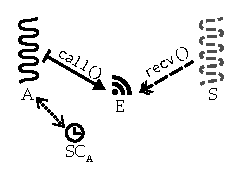
\includegraphics[width=\textwidth]{passive1}
        \caption{Phase 1}
        \label{f:passive1}
    \end{subfigure}%
    \begin{subfigure}[h]{0.48\textwidth}
        \centering
        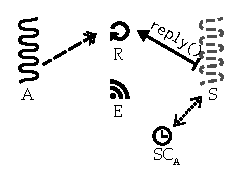
\includegraphics[width=\textwidth]{passive2}
        \caption{Phase 2}
        \label{f:passive2}
    \end{subfigure}
    \caption[IPC phases between an active client and passive server.]{IPC phases between an active client and passive server: (a) shows the initial IPC rendezvous, (b) shows the
    reply phase. The client's $SC_{A}$ is donated between client and server. See \Cref{f:legend-2} for the legend.}
    \label{f:passive}
\end{figure}
\begin{figure}
\centering
\begin{subfigure}[h]{0.48\textwidth}
    \centering
    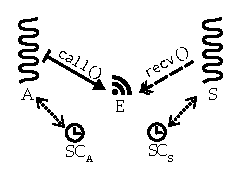
\includegraphics[width=\textwidth]{active1}
    \caption{Phase 1}
    \label{f:active1}
\end{subfigure}%
\begin{subfigure}[h]{0.48\textwidth}
    \centering
    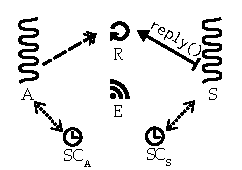
\includegraphics[width=\textwidth]{active2}
    \caption{Phase 2}
    \label{f:active2}
\end{subfigure}
\caption[IPC phases between active client and active server.]{IPC phases between an active client and active server: (a) shows the initial IPC rendezvous, (b) shows the
reply phase. Both client and server have their own SC. See \Cref{f:legend-2} for the legend.}
\label{f:active}
\end{figure}

Charging for time executed in a server is simple in our model: charge the scheduling
context that the resource server is running on.
The question is, \emph{which} scheduling context is the server running on? Unlike
previous implementations of donation like semantics, our model does not mandate
scheduling context donation. Resource servers are free to run on their own scheduling context, 
according to the policy of the system.

Whether donation occurs or not is inferred at the time of the IPC rendezvous: we test if the
server is passive or active. 
\emph{Passive} servers do not have a scheduling context 
and receive them over \gls{IPC} whereas \emph{active} servers have their own scheduling context. 
Passive servers, as illustrated in \cref{f:passive}, effectively provide a migrating-thread
model~\citep{Ford_Lepreau_94, Gabber_SBBS_99}, but without requiring
the kernel to manage stacks. \Cref{f:active} shows active servers, which allow system designers to
build systems without temporal isolation, as it is not suitable
for all systems.

\subsection{Enforcement}

If a passive resource server exhausts the scheduling context it is running on, it and any waiting clients
are blocked until replenishment. On its own, this means that a client
not only has to trust its server, but all the server's other
clients. This would rule out sharing a server between clients of
different criticality.

In a \gls{HRT} system, we can assume that a client's reservations are sufficient to complete
requests to servers.  However, in systems with best-effort and soft real-time tasks, no such
assumption can be made and client budgets may expire during a server request.  This leaves the
server in a state where it cannot take new requests as it is stuck without an active reservation to
complete the previous request.  Without a mechanism to handle this event the server, and any
potential clients, would be blocked until the client's budget is replenished.

Timeout exceptions can be used to remove this need for trust, and
allow a server to be shared across criticalities, as depicted in \cref{f:timeout}. Timeout fault endpoints are specific to the
execution context of a thread, not the scheduling context. Consequently, servers may have timeout
fault handlers while clients do not. The 
server's timeout handler can, for example, provide an emergency budget
to continue the operation (useful for \crit{HI} clients) or abort
the operation and reset or roll back the server. The latter option is
attractive for minimising the amount of budget that must be reserved
for such cases.

\begin{figure}
    \centering
    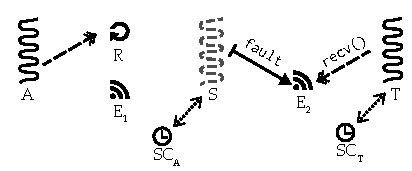
\includegraphics[width=0.8\textwidth]{timeout}
    \caption[Example of a timeout exception handler.]{Example of a timeout exception handler. The passive server $S$ performs a request on
    client $A$'s scheduling context, $SC_{A}$. A timeout fault is generated when $SC_{A}$ is
exhausted and sent to the server's timeout fault endpoint $E_{2}$, and the timeout handler receives
it. See legend \cref{f:legend-2}}
    \label{f:timeout}
\end{figure}


A server running out of budget constitutes a protocol violation
by the client, and it makes sense to penalise that
client by aborting. Helping schemes, such as \gls{PIP} or bandwidth
inheritance,
make the waiting client pay for
another client's contract violation. This not only weakens temporal isolation,
it also implies that the size of the required reserve budget
must be a server's full WCET. This places a restriction on the server
that no client request exceed a blocking time that can be tolerated by
all clients, or that all clients must budget for the full server WCET in
addition to the time the server needs for serving their own request.
Our model provides more flexibility: a server can use a timeout
exception to finish a request early (e.g.\ by aborting), meaning that clients can only be
blocked by the server's \gls{WCET} (plus the short
clean up time).

\subsection{Multiprocessors}

The mechanism of scheduling-context donation can also be used across processing cores, and 
allows users to easily specify if servers should migrate to the core of the client, or 
process the request on a remote core. Specifically, active servers process requests on the core of
their own scheduling context, and passive servers migrate to the scheduling context of the client. 
The mechanism is simple: if a
server is passive, it migrates to the core that the donated scheduling context provides time for. 

\section{Mechanisms}
\label{sec:model-mechanisms}

Before exploring how various user-level policies can be implemented using our model, we describe
four new mechanisms introduced for high-performance implementation of those policies.

\subsection{Directed yield}

The first is simple: in order to implement user-level schedulers, the kernels scheduling queues
must be able to be manipulated. For this, we add an operation on scheduling contexts: a
directed yield to a specific scheduling context. By invoking the \scyieldto invocation on 
a specific scheduling context, the thread running on that scheduling context is placed at the head
of the scheduler queue for its priority. 
This may change the currently running thread if it is at the same priority, and only effects the
scheduler if there is a runnable thread bound to the invoked scheduling context. Threads cannot
yield to threads of higher priorities than their own, as they are by definition, not currently
running.

\subsection{IPC Forwarding}
\label{sec:ipc-forwarding}

We introduce another concept called \emph{forwarding}, which allows callers to
invoke one capability and block on another capability in the same system call, via
a new system call \nbsendrecv. This is required to
facilitate a forwarding IPC, and allows passive proxies to seamlessly forward messages,
capabilities and scheduling contexts, as shown in \cref{f:model-forward}. 

\begin{figure}
    \centering
    \begin{subfigure}[h]{0.8\textwidth}
        \centering
        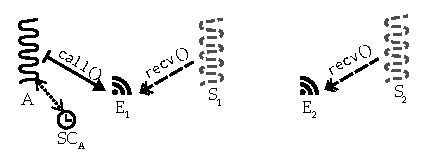
\includegraphics[width=\textwidth]{forward1}
        \caption{$A$ \call() $S_{1}$ over $E_{1}$.}
        \label{f:forward1}
    \end{subfigure}
    \begin{subfigure}[h]{0.8\textwidth}
        \centering
        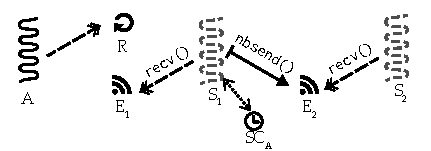
\includegraphics[width=\textwidth]{forward2}
        \caption{$S_{1}$ uses \nbsendrecv() to forward the request, and $A$'s resume 
            capability, to $E_{2}$, and
        wait for further messages on $E_{1}$.}
        \label{f:forward2}
    \end{subfigure}
    \begin{subfigure}[h]{0.8\textwidth}
        \centering
        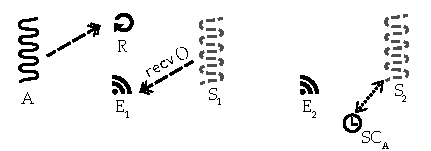
\includegraphics[width=\textwidth]{forward3}
        \caption{$S_{2}$ processes the request.}
        \label{f:forward3}
    \end{subfigure}
    \begin{subfigure}[h]{0.8\textwidth}
        \centering
        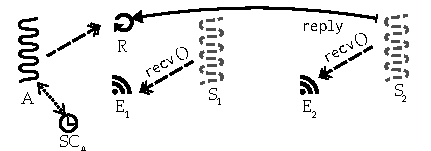
\includegraphics[width=\textwidth]{forward4}
        \caption{$S_{2}$ uses the \replyrecv() system call to reply to $A$ and block on
        $E_{2}$ again. }
        \label{f:forward4}
\end{subfigure}
\caption[IPC forwarding.]{IPC forwarding: client $A$ sends a request to passive server $S_{2}$ via a passive proxy $S_{1}$,
and the scheduling context passes from $A \rightarrow S_{1} \rightarrow S_{2} \rightarrow A$. See \Cref{f:legend-2} for the legend.}
\label{f:model-forward}
\end{figure}

\subsection{Flexible Resume Capabilities}

The final mechanism we introduce is the ability to transfer resume capabilities between servers. 
This means that a blocked thread can be forwarded to other threads, thus allowing the resume
capability to be moved. Note that this is explicitly not delegation: resume capabilities cannot be
copied.

\subsection{Notification Binding}

Recall from \cref{s:notification-binding} that notification objects can be bound to threads such that single-threaded servers can be 
constructed which receive IPC messages and signals. We extend this mechanism with passive server
support by allowing scheduling contexts to be bound to notifications, such that the passive server
execute using the notification's scheduling context when processing interrupts or signals from other
threads. 

\section{Policies}
\label{sec:model-policies}

We now describe how different policies can be implemented by user-level systems using the 
existing mechanisms in seL4, combined with the new mechanisms of scheduling contexts,
scheduling context donation, directed yield, IPC forwarding, and flexible resume capabilities.
First, we explain how different best-effort, rate-based and real-time tasks are compatible
with our model and describe their implementation. We subsequently explain how various different 
resource sharing policies and servers, with and without temporal isolation, can be constructed. 

\subsection{Scheduling policies}

\subsubsection{Best-effort threads}

Best-effort threads, scheduled round-robin, are compatible with our model, which maintains
compatibility with the previous, baseline \selfour scheduler.  Full scheduling contexts are the
mechanism to support best-effort threads, and by setting the budget and period to equal, system
designers can set a timeslice, which determines how long a specific scheduling context can be
executed upon before preemption.

More complicated, time-sharing schedulers can be built by a user level scheduler, using the directed
yield and ability to request the amount of time consumed by a specific scheduling context.

\subsubsection{Rate-limited threads}

Rate-limited threads simply have their scheduling contexts configured with
parameters that express the desired upper-bound on rate.  No other work is
required by the user: if there are no higher priority threads and the
rate-limited thread does not block, it will be runnable at the rate expressed
in the scheduling context.  Otherwise, the thread will be capped at the rate
specified, but cannot be guaranteed to get the entire rate allocation if there
are higher priority threads in the system, or if the priority of the
rate-limited thread is overloaded.

\subsubsection{Periodic, polling threads}

Threads that need to wake, poll for an event, and sleep again can be
implemented using the sporadic server mechanism, by  
setting threads' scheduling parameters appropriately. As long as the budget is
not full ($C\neq T$), the \yield system call can be used to block until the next replenishment
is available, as shown in \cref{list:polling}. However, this approach will only work if the amount of thread preemptions 
is known and the amount of extra sporadic replenishments is set correctly, as \yield sleeps until
the next available replenishment. If fragmentation occurs due to preemption and incorrect sporadic
replenishments, the polling thread will not wake at the start of every period. This could be
ameliorated by checking the time on wakeup, or using a different task model.  

\begin{listing}
  \begin{minted}{c}
      for (;;) {
          seL4_Word badge;
          seL4_Poll(notification_object, &badge);
          doJob();
          // sleep until next job is ready
          seL4_Yield();
      }
  \end{minted}
  \caption{Example of a polling task on \selfour.}
  \label{list:polling}
\end{listing}

\subsubsection{Sporadic threads}

For sporadic threads, which wake due to an event, process and sleep again and may be subject to a
maximum CPU bandwidth, notifications combined
with scheduling contexts can be used, as displayed in \cref{list:model-sporadic}. In this case, if the
number of sporadic replenishments is not sufficient, the processing bandwidth may be artificially
limited by excessive preemptions, otherwise it will be $\frac{C}{T}$. 

\begin{listing}
  \begin{minted}{c}
      for (;;) {
          doJob();
          // sleep until next job is ready
          seL4_Word badge;
          seL4_Wait(notification_object, &badge);
      }
  \end{minted}
  \caption{Example of a basic sporadic task on \selfour.}
  \label{list:model-sporadic}
\end{listing}

\subsubsection{Time triggered threads}

Time-triggered threads, which wake up, do some processing, and go to sleep again until the next
period can be set up with a user-level timer driver in order to wake at exactly the right time.
Scheduling contexts can be combined with this approach to rate-limit time-triggered threads, but 
the exact amount of preemptions does not need to be known.
\cref{list:model-sporadic} also applies to this policy, where the notification object is configured to
receive periodic notifications from a timer service.

\subsubsection{EDF scheduling}

\TODO{How to do EDF}

\subsubsection{CFS scheduling}

\TODO{How to do CFS}

\subsection{Resource sharing policies}

\subsubsection{\gls{PIP}/\gls{BWI}}
\label{sec:model-pip-bwi}

\begin{figure}
    \centering
    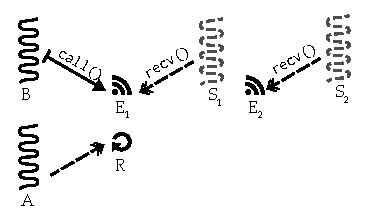
\includegraphics[width=0.7\textwidth]{pip}
    \caption[Example of proxying requests via a server.]{Example of proxying requests via a server that manipulates priorities before resource
    access, see \cref{f:legend-2} for the Legend.}
    \label{f:model-pip}
\end{figure}
 
\cref{f:model-pip} shows an example of a resource server ($S_{2}$) which proxies IPC messages via
another server ($S_{1}$) to manipulate priorities according to some protocol before and after
requests. The policy works as follows: clients are given a badged capability to an endpoint,
$E_{1}$, on which to make requests on the resource server. $S_{1}$ receives requests, identifies 
the client via the badge, and manipulates $S_{2}$'s priority before forwarding the request to
$S_{2}$ over endpoint $E_{2}$. $S_{1}$ returns to wait on $E_{1}$, while $S_{2}$ processes the
request. If while $S_{2}$ is processing a request from $A$, and a higher priority thread $B$
preempts it and sends a request on $E_{1}$, $S_{2}$ can bump $S_{1}$'s priority again, and forward
$B$'s request to $S_{2}$, once again returning to wait on $E_{1}$ for further messages. When $A$'s
request is complete, $S_{2}$ enqueues a request on $E_{1}$, such that $S_{1}$ can readjust the
priority of $S_{2}$ according to the protocol, and reply to the original caller. Note that for this
method to work, $S_{1}$ must be the highest priority, and acts as a critical section for
manipulating priorities in the system.

Our description so far can be used to implement the \gls{PIP} or the \gls{OPCP}, depending on 
the logic used by the proxy-server $S_{1}$. This functions whether $S_{1}$ and $S_{2}$ are active or
not. In order to extend this protocol to bandwidth inheritance, a timeout fault handler would need
to be specified for both server threads, which could then bind the pending client's scheduling
context to the server to finish the request. 

\subsubsection{Best-effort Shared Server}
\label{sec:best-effort}

Best-effort systems have no timing requirements, so each thread in the system has a full \gls{SC}
with a budget and period the length of the timeslice. Threads are scheduled round-robin. To
implement such a system with our mechanisms, all server threads would be configured as active, and 
set to the ceiling priority of the clients. 

This policy does not provide temporal isolation, as the server executes on its own budget.  If one
client launches a denial of service attack on the server, depleting the servers budget, then other
clients are starved. 

While our resource sharing mechanisms do not rule out this policy, it is only suitable for
systems where all clients are trusted and the amount of requests each client makes is known \emph{a
priori}, or systems that have low temporal sensitivity.

\subsubsection{Migrating threads}

\composite~\citep{Parmer_10} solves the resource sharing model by using migrating 
threads (also termed stack-migrating IPC).
On every IPC, client execution contexts (and CPU reservation) transfer to a new stack running in the
server's protection domain, resulting in multi-threaded servers.

To implement migrating threads, \composite requires that every server have a mechanism for allocating stacks.
If no memory is available to allocate stacks, then the request is blocked.
This solution forces servers to be multi-threaded, and does not solve the problem of a clients budget expiring while the server is in a critical section, which is solved by providing atomic primitives that call the kernel.

A stack-spawning policy can be implemented using the mechanisms we have provided, similarly to
the \gls{PIP} implementation described above (\cref{sec:model-pip-bwi}), except the proxy
server spawns new worker threads instead of manipulating priorities. 
The stack-spawning proxy would also be at a lower priority than the worker threads, 
such that it would only be activated when all worker threads are busy.

An alternative policy is to build systems with a fixed number of server threads, all waiting on the
same endpoint. 
Like the best-effort policy, our model supports this approach but it is not required.

\subsubsection{Blocking Servers}

Some servers need to block in order to function: for example, servers providing \IO may need to wait
until an operation completes before replying to the client. Consider a disk server, where
clients make requests of the server to write data to the disk. The server makes the request to the
disk, but does not reply to the client until the device has signalled that \IO is complete. Rather
than blocking until the driver responds, preventing the server from taking on further requests, the
server can block on the endpoint and wait for the interrupt or further RPC requests. If an interrupt
comes in, the server runs the bound notification objects scheduling context to complete the
request.

Another option is to use multiple threads, with a passive thread for handling requests and an active
thread servicing interrupts, however this requires synchronisation between the threads within the
server.

\subsubsection{Server isolation}

We now describe how timeout handlers can be used to implement server isolation and other policies,
as previously introduced in \cref{sec:model-enforcement}. 

For our example consider a server shared between clients of different criticality, time sensitivity,
and trust, which provides an encryption service via \gls{AES}. 
Such a server processes data in blocks, and the \gls{WCET} of a request is a function of the 
amount of data to be encrypted. Such a server can be constructed transactionally in order
to render it preemptable: each block processes is considered a transaction. The server atomically
switches between two states each time it completes a block, effectively finishing one transaction
and starting another. The state the server is working on is always dirty, the previous is clean. 

By constructing the server in this way, a timeout handler can reset the server to the last clean
state if the passive server raises a timeout exception due to the client's \gls{SC} expiring. 
The timeout handler saves the server at a known checkpoint, and flips the server back to 
the known checkpoint. The handler can then reply to the client on the server's behalf, and return how
far through the request the server completed by reading it out of the last clean state. Invoking the
reply returns the scheduling context to the client, and the timeout handler blocks waiting for the
next request.

Other options are also available to the timeout handler, which is important as not all server
operations can be reset midway. The timeout handler can reply with an error to the client, 
not reply to the client at all, thereby preventing the client from making further requests, or 
bind a temporary scheduling context to the server to complete the request. 

\section{Summary}

In this chapter we have outlined our model for providing temporal isolation via scheduling and
resource sharing mechanisms. We introduce support for user-level
admission tests via a new control capability, and add processor reservations to the kernel in the form of scheduling contexts.  
Scheduling contexts differ from prior work in that they are decoupled from priority, thereby
avoiding priority inheritance on scheduling context donation, and by differentiating between passive and active servers we maintain policy freedom.

Finally, we outlined existing models for integrating real-time resource policies over \gls{IPC} and
show how scheduling-context donation combined with passive servers can be used to create trusted
servers with untrusted clients. 
Our model supports best-effort, migrating threads, or temporal isolation policies for resource sharing.

Timeout exceptions are provided which allow for user-defined enforcement policies, while the default
mechanism maintains isolation by preventing threads from executing for than the share of processing
time represented by the scheduling contexts.

In the next section we will outline the implementation of our model in \selfour. 
